\documentclass{emulateapj}
%\documentclass[12pt,preprint]{aastex}

\usepackage{hyperref}

\usepackage{graphicx}
\usepackage{float}
\usepackage{amsmath}
\usepackage{epsfig,floatflt}
\usepackage{listings}
\usepackage{gensymb}
\usepackage{upgreek}
\usepackage{csquotes}
\usepackage{color}
% \usepackage{natbib}


\lstset{frame=tb,
  language=Python,
  aboveskip=3mm,
  belowskip=3mm,
  showstringspaces=false,
  columns=flexible,
  basicstyle={\small\ttfamily},
  numbers=none,
  numberstyle=\tiny\color{gray},
  keywordstyle=\color{blue},
  commentstyle=\color{dkgreen},
  stringstyle=\color{mauve},
  breaklines=true,
  breakatwhitespace=true,
  tabsize=3
}

\newcommand\p[2]{\frac{\partial #1}{\partial #2}}
\newcommand\Lag[1]{\frac{d}{dt}\left( \dfrac{\partial L}{\partial \Dot{#1}}\right) - \dfrac{\partial L}{\partial #1} &= 0}


\begin{document}

\title{Computational Physics - Project 1}

\author{
  Dahl, Jon Kristian \\
  \and
  Sand, Mats Ola \\
  \and
  Fløisand, Johan Andreas \\
}

\begin{abstract}
Yes
\end{abstract}
 
%%%%%%%%%%%%%%%%%%%%%%%%%%%%%%%%%%%%
%%%%%%%%%%%%%%%%%%%%%%%%%%%%%%%%%%%%
\section{Introduction}
%%%%%%%%%%%%%%%%%%%%%%%%%%%%%%%%%%%%
%%%%%%%%%%%%%%%%%%%%%%%%%%%%%%%%%%%%
Linear algebra naturally occurs in computational physics due to problems where continuous parameters needs to be discretized. Natural examples of this are differential equations which are not analytically solvable that needs to be solved numerically. In this report we will solve the Poisson equation \cite[Chapter 13]{matmet}, \(-\frac{d^2u}{dx^2} = f(x)\), by discretizing it into a linear algebra problem which can be solved by a simple matrix equation. We will solve the matrix equation using three different algorithms and then compare the relative numerical error and computation time between them each of them.

The three algorithms are: The Thomas algorithm for a general tridiagonal matrix, a Thomas algorithm specially designed for the matrix representing the Poisson equation (i.e., a tridiagonal T\"{o}plitz matrix), and lastly LU decomposition for a dense matrix.
\newline
\newline
We begin with a method section where we introduce the differential equation and explain the algorithms. The results section follows where we compare the relative errors and computation times of the algorithms. Finally, we discuss our results and conclude how each algorithm fits different purposes.
%%%%%%%%%%%%%%%%%%%%%%%%%%%%%%%%%%%%
%%%%%%%%%%%%%%%%%%%%%%%%%%%%%%%%%%%%
\section{Method}
%%%%%%%%%%%%%%%%%%%%%%%%%%%%%%%%%%%%
%%%%%%%%%%%%%%%%%%%%%%%%%%%%%%%%%%%%
Lets now introduce the Poisson equation and show how we can find an expression for the double derivative of a function using Taylor series \cite[Chapter 11]{kalkulus}.
%We introduce the Poisson equation and show how we can find an expression for the double derivative of a function using Taylor series. We show how this can be discretized into a single tridiagonal matrix equation which can be solved by the Thomas algorithm. Since the matrix is a T\"{o}plitz matrix
%Finally we show that we can also use the standard LU decomposition and .
%%%%%%%%%%%%%%%%%%%%%%%%%%%%%%%%%%%%
\subsection{The Poisson equation}
%%%%%%%%%%%%%%%%%%%%%%%%%%%%%%%%%%%%
The Poisson equation pops up in several problems in physics, for instance in the electrostatic potential \(\Phi\):

\begin{equation*}
    \nabla^2\Phi = -4\pi\rho(\mathbf{r}).
\end{equation*}
Assuming that the electrostatic potential only depends on the radial distance \(r\), a few lines of algebra shows that we get back the Poisson equation \cite[Chapter 13]{matmet}, \(\frac{d^{2}\phi(r)}{dr^{2}}=-4\pi r\rho(r)\). Rewriting \(\phi\rightarrow u\) and \(r\rightarrow x\) we are left with:

\begin{equation}\label{eq:Poisson_equation}
    -\frac{d^{2}u(x)}{dx^{2}} = g(x).
\end{equation}
To see how the errors of the different algorithms unfold, we can choose \(g\) such that an exact solution for \(u\) exists. We apply our function \( u \) on the interval \([0,1]\) with the Dirichlet boundary conditions \cite[Chapter 13]{matmet}, that is \(u(0) = u(1) = 0\). Choosing

\begin{equation*}
    g(x) = 100e^{-10x},
\end{equation*}
which has the exact solution

\begin{equation*}
    u(x) = 1 - \left(1 - e^{-10}\right)x - e^{-10x},
\end{equation*}
for the given boundary conditions, the relative error can be computed. To see this, we plug it back into the Poisson equation:

\begin{align*}
    -\frac{d^{2}u(x)}{dx^{2}} &= 
    \frac{d^{2}}{dx^{2}}(-1) + \frac{d^{2}}{dx^{2}}\left(1 - e^{-10}\right)x + \frac{d^{2}}{dx^{2}}e^{-10x} \\
    &= \frac{d}{dx}\left(1 - e^{-10}\right)+  \left(-10\right)^{2}e^{-10x} \\
    &= 100e^{-10x} = g(x).
\end{align*}
We also have 

\begin{align*}
    u(0) &= 1 - \left(1 - e^{-10}\right)\cdot0 - e^{-10\cdot0} 
    = 1 - e^{0} = 0 \\
    u(1) &= 1 - \left(1 - e^{-10}\right)\cdot1 - e^{-10\cdot1} 
    = e^{-10} - e^{-10} = 0 
\end{align*}
%%%%%%%%%%%%%%%%%%%%%%%%%%%%%%%%%%%%
\subsection{Approximation of the second derivative}
%%%%%%%%%%%%%%%%%%%%%%%%%%%%%%%%%%%%
The Taylor series of a function \(f\) about the point \(a\) is given by (see \cite[Chapter 11]{matmet})

\begin{equation*}
    f(x) = \sum_{n=0}^{\infty}\frac{1}{n!}\left(x-a\right)^{n}f^{(n)}(a),
\end{equation*}
where we define \(f^{(n)}(a)\) for \(n\in\mathbb{N}\cup\{0\}\) as the \(n\)th derivative of \(f\) evaluated at \(a\). Using \textquote{Big O} notation, we write the series as

\begin{equation*}
    f(x) = \sum_{n=0}^{k}\frac{1}{n!}\left(x-a\right)^{n}f^{(n)}(a) + \mathcal{O}\big((x-a)^{k}\big),
\end{equation*}
where \(\mathcal{O}\big((x-a)^{k}\big)\) contains the rest of the series. Assuming that the value \(x\) is fairly close to \(a\), the leading term of the rest will go as \((x-a)^{k}\). Thus, we can approximate the series as 

\begin{equation*}
    f(x) \approx \sum_{n=0}^{k}\frac{1}{n!}\left(x-a\right)^{n}f^{(n)}(a),
\end{equation*}
with an error of order \(\mathcal{O}\big((x-a)^{k}\big)\).

If we now chose \(x = x + h\) and \(a = h\), we find

\begin{equation*}
    f(x+h) = f(x) + hf^{\prime}(x) + \frac{1}{2!}h^{2}f^{\prime\prime}(x) + \frac{1}{3!}h^{3}f^{\prime\prime\prime}(x) + \mathcal{O}_{1}\big(h^{4}\big).
\end{equation*}
For \(x = x - h\) and \(a = h\), we have

\begin{equation*}
    f(x-h) = f(x) - hf^{\prime}(x) + \frac{1}{2!}h^{2}f^{\prime\prime}(x) - \frac{1}{3!}h^{3}f^{\prime\prime\prime}(x) + \mathcal{O}_{2}\big(h^{4}\big).
\end{equation*}
Adding the two equation gives

\begin{equation*}
    f(x+h) + f(x-h) = 2f(x) + h^{2}f^{\prime\prime}(x) + \overbrace{\mathcal{O}_{1}\big(h^{4}\big) + \mathcal{O}_{2}\big(h^{4}\big)}^{\mathcal{O}\big(h^{4}\big)}.
\end{equation*}
Solving for the double derivative we have

\begin{equation}\label{eq:f_double_derivative_taylor}
    f^{\prime\prime}(x) = \frac{f(x+h) - 2f(x)+ f(x-h)}{h^{2}} + \mathcal{O}\big(h^{2}\big).
\end{equation}
%\newline
%\newline
%\newline
%where we define \(f^{n}\) for \(n\in\mathbb{N}\cup\{0\}\) as the composition of \(f\) with itself \(n\) times. That is 
%\begin{equation*}
%    f^{n}(x) = \overbrace{(f\circ f\circ\ldots\circ f)}^{n\text{ times}}(x) = \overbrace{f(f(\ldots(f}^{n\text{ times}}(x))\ldots))
%\end{equation*}
%%%%%%%%%%%%%%%%%%%%%%%%%%%%%%%%%%%%
\subsection{Discretizing and setting up a matrix equation}
%%%%%%%%%%%%%%%%%%%%%%%%%%%%%%%%%%%%
Our function can not be represented continuously on a computer. Hence we need to discretize the problem. To see how we can do this we will choose to discretize the interval \([a,b]\) with \(N\) points. If we choose linearly spaced points we will have a stepsize \(h = \frac{b - a}{n}\) and we define 
\begin{align*}
    &f_{0}=f(0\cdot h),\quad f_{1}=f(1\cdot h),\quad f_{2}=f(2\cdot h),\quad \ldots,\\ &f_{n-1}=f((n-1)\cdot h),\quad f_{n}=f(n\cdot h).
\end{align*}

We recognize the Poisson equation (\ref{eq:Poisson_equation}) by its Taylor series
\begin{equation}\label{eq:f_double_derivative_taylor}
    -u^{\prime\prime}(x) = \frac{-u(x+h) + 2f(x) - f(x-h)}{h^{2}} + \mathcal{O}\big(h^{2}\big) = g(x),
\end{equation}
which we now can discretize for an \(x=i\cdot h\):
\begin{align}\label{eq:f_double_derivative_discrete}
    -\dfrac{v_{i+1} + v_{i-1} - 2v_{i}}{h^{2}} &= g_{i}\nonumber
    \\
    -v_{i-1} + 2v_{i} - v_{i+1} &= h^{2} g_{i}.
\end{align}
We have changed the function \(u\) to \(v\) to indicate that we do not have an exact solution, but for large \(N\) the error goes as \(\mathcal{O}\big(h^{2}\big)\). 

%%%%%%%%%%%%%%%%%%%%%%%%%%%%%%%%%%%%
\subsection{Rephrasing as a linear algebra problem}
%%%%%%%%%%%%%%%%%%%%%%%%%%%%%%%%%%%%

For \(i=0\), equation (\ref{eq:f_double_derivative_discrete}) becomes

\begin{equation*}
    -v_{-1} + 2v_{0} - v_{1} = h^{2} g_{0},
\end{equation*}
which we can not solve since our boundary conditions tells us that \(u_{0}=u_{n}=0\), and nothing about \(u_{-1}\). We run into the same problem for \(i=n\). For \(0 < i < n\), we can write ut the equations:

\begin{align*}
    2v_{1} - v_{2} &= h^{2} g_{1} \\
    -v_{1} + 2v_{2} - v_{3} &= h^{2} g_{2} \\
    -v_{2} + 2v_{3} - v_{4} &= h^{2} g_{3} \\
    &\vdots \\
    -v_{n-3} + 2v_{n-2} - v_{n-1} &= h^{2} g_{n-2} \\
    -v_{n-2} + 2v_{n-1} &= h^{2} g_{n-1},
\end{align*}
and this is nothing else but a matrix product, \(\textbf{A}\textbf{v} = \widetilde{\textbf{g}}\), where the left-hand-side of equation (\ref{eq:f_double_derivative_discrete}) represents \(\textbf{A}\textbf{v}\) and the right-hand-side represents \(\widetilde{\textbf{g}}\). The matrix \(\textbf{A}\) is a tridiagonal T\"oplitz matrix

\begin{equation}
\mathbf{A} = \begin{bmatrix}
                   2      & -1     & 0      & \ldots & \ldots & \ldots & 0      \\
                   -1     & 2      & -1     & 0      & \ldots & \ldots & \vdots \\
                   0      & -1     & 2      & -1     & 0      & \ldots & \vdots \\
                   \vdots &        & \ddots & \ddots & \ddots & \vdots & \vdots \\
                          &        &        & \ddots & \ddots & \ddots &        \\
                   0      & \ldots & \ldots & 0      & -1     & 2      & -1     \\
                   0      & \ldots & \ldots & \ldots & 0      & -1     & 2      \\
              \end{bmatrix}.
\end{equation}
Using only the fact that this matrix is tridiagonal, we can use the Thomas algorithm to solve the matrix equation.

%%%%%%%%%%%%%%%%%%%%%%%%%%%%%%%%%%%%
\subsection{Thomas algorithm}
\label{sec:thomas}
%%%%%%%%%%%%%%%%%%%%%%%%%%%%%%%%%%%%

The Thomas algorithm is an algorithm for row reducing tridiagonal matrices. 
In a tridiagonal matrix all elements are zero, except for the diagonal and the elements directly above and below the diagonal. Our matrix equation thus looks like

\begin{equation*}
    \mathbf{A}\mathbf{v} = \begin{bmatrix}
       b_1    & c_1    & 0      & \ldots  & \ldots  & 0 \\
       a_1    & b_2    & c_2    & 0       & \ldots  & \vdots \\
       0      & a_2    & b_3    & c_3     & \ddots  & \vdots \\
       \vdots & \ldots & \ddots & \ddots  & \ddots  & \vdots \\
       \vdots & \ldots & \ldots & a_{n-3} & b_{n-2} & c_{n-2} \\
       0      & \ldots & \ldots & \ldots  & a_{n-2} & b_{n-1} \\
    \end{bmatrix}\begin{bmatrix}
        v_1\\
        v_2\\
        \vdots \\
        \vdots  \\
        \vdots \\
        v_{n-1}\\
    \end{bmatrix}
    =\begin{bmatrix}
        h^{2}g_{1} \\
        h^{2}g_{2} \\
        \vdots      \\
        \vdots      \\
        \vdots      \\
        h^{2}g_{n-1} \\
    \end{bmatrix}.
\end{equation*}

In C++, the algorithm for solving the above equation reads

\begin{lstlisting}
for (int i=0; i<n-1; i++)
    {
        diag[i+1] = diag[i+1] - lower_diag[i]/diag[i]*upper_diag[i];
        rhs_val[i+1] = rhs_val[i+1] - lower_diag[i]/diag[i]*rhs_val[i];
    }

for (int i=n-1; i>=1; i--)
    {
        computed[i-1] = (rhs_val[i-1] - upper_diag[i-1]*computed[i])/diag[i-1];
    }
\end{lstlisting}
%Forward backward subst
where diag, lower\_diag and upper\_diag are the arrays storing the diagonal, lower diagonal, and upper diagonal elements respectively. From this code snippet we can count the additions and multiplications and sum it up to be 9 FLOPS. The algorithm is constructed by first doing a forward and then a backward substitution. That is: Firstly, the elements in the lower diagonal, denoted \( a_i\), needs to be turned into zeros by means of row reduction. This is achieved by initially subtracting the first row multiplied by some factor, from the second row. This factor must be \( b_1/a_1 \) for \( a_1 \) to become zero. We observe that in this process the diagonal element \( b_2 \) and the element \( h^2g_2 \) will be changed.

The next step is to eliminate \(a_2\), and that process will be equivalent to that of \(a_1 \), hence we have the general case seen in the above code in the first for loop. Since all the elements in the lower diagonal becomes zero, there is no need to actually compute them.

When all the lower diagonal elements are dealt with, we need to do the same with the upper diagonal elements denoted \( c_i \). We achieve this by first subtracting the last row times some factor, from the second last row. This factor is, similarly to the lower diagonals, \( c_{n-2}/b_{n-1} \). When this is applied to all the upper diagonal elements, we need to divide each row (which now only consist of diagonal elements) by its diagonal element, and read out the computed values, v. This step can be done more compactly as in the second for loop in the above code. We now have the advantage that the bottom row is already solved. It consists only of a single known value which will be used when eliminating the above upper diagonal element. If we look at the computer code for this process, it reads

\begin{align}
    h^2g_{n-2} &= b'_{n-2}v_{n-2} + c_{n-2}v_{n-1},
    \\ \label{eq:thomas_final}
    v_{n-2} &= (h^2g'_{n-2} - c_{n-2}v_{n-1})/b_{n-2},
\end{align}{}
showing that we can shorten the actual calculation, saving computer resources. The prime values indicate that the value earlier has been changed from its non-prime state during the row reduction. Equation \ref{eq:thomas_final} is the final step of the Thomas algorithm, and by this, the matrix equation is solved.


\subsection{Specialized Thomas algorithm}
\label{sec:special_thomas}

    The specialized Thomas algorithm comes from the fact that we know the value of the tridiagonal elements.
    
    \begin{lstlisting}
        for (int i=0; i<n-1; i++)
            {
                diag[i+1] = 2.0 - 1.0/diag[i];
            }
    \end{lstlisting}{}
    In this code snippet, we use that the diagonal elements are all 2, and the upper and lower diagonals are all -1, so that we don't need to fetch these values from memory. This leads to the simplified versions of the forward and backwards substitutions from the normal Thomas algorithm:
    
    \begin{lstlisting}
        for (int i=0; i<n-1; i++)
            {
                rhs_val[i+1] = rhs_val[i+1] + rhs_val[i]/diag[i];
            }
            
        for (int i=n-1; i>=1; i--)
            {
                computed[i-1] = (rhs_val[i-1] + computed[i])/diag[i-1];
            }
    \end{lstlisting}{}
    Here, we can count the number of floating point operations to be 4 per iteration, as compared to the 9 from the normal Thomas algorithm.

%%%%%%%%%%%%%%%%%%%%%%%%%%%%%%%%%%%%
\subsection{LU decomposition}
%%%%%%%%%%%%%%%%%%%%%%%%%%%%%%%%%%%%

Till now we have looked at the Thomas algorithm which requires tridiagonal matrices. If we now loosen the requirement and let \(\textbf{A}\) be a dense matrix, we would need a new way of solving the matrix equation. An excellent method for doing this is to first LU decompose \(\textbf{A}\) and then solving for the unknown vector \(\textbf{v}\).

LU decomposition (described in \cite[Chapter 2]{linalg} and \cite[Chapter 6]{compfys}) requires that \(\textbf{A}\) has no singular values along its diagonal, but if it does, one can if possible permute the rows of \(\textbf{A}\) such that the requirement is met and remember how the rows are permuted when the equation is solved and permute back. The decomposition uses normal gaussian elimination (row reduction) of a dense matrix 

\begin{equation*}
    \mathbf{A} = \begin{bmatrix}
       a_{11} & a_{12} & \ldots & a_{1n} \\
       a_{21} & a_{22} & \ldots & a_{2n} \\
       \vdots & \vdots & \ddots & \vdots \\
       a_{n1} & \ldots & \ldots & a_{nn} \\
    \end{bmatrix},
\end{equation*}
to create a lower triagonal matrix \(\textbf{L}\) and an upper triangular matrix \(\textbf{U}\),

\begin{align*}
    \textbf{A} &= \textbf{L}\textbf{U} =
    \begin{bmatrix}
       l_{11} & 0      & \ldots & \ldots & 0      \\
       l_{21} & l_{22} & 0      & \ldots & 0      \\
       \vdots & \vdots & \ddots &        & \vdots \\
       \vdots & \vdots &        & \ddots & 0      \\
       l_{n1} & l_{n2} & \ldots & \ldots & l_{nn} \\
    \end{bmatrix}
    \begin{bmatrix}
       u_{11} & u_{12} & \ldots & \ldots & u_{1n} \\
       0      & u_{22} & \ldots & \ldots & u_{2n} \\
       \vdots & 0      & \ddots &        & \vdots \\
       \vdots & \vdots &        & \ddots & \vdots \\
       0      & 0      & \ldots & \ldots & u_{nn} \\
    \end{bmatrix}.
\end{align*}
Without loss of generality, we can choose \(l_{ii}=1\) for \(i=1,\,2,\ldots,n\). 

Our simplified matrix equation now looks like

\begin{align*}
    \textbf{L}\textbf{U}\textbf{v} &= \widetilde{\textbf{g}} \\
    \textbf{L}\textbf{z} &= \widetilde{\textbf{g}}
\end{align*}
where \(\widetilde{\textbf{g}} = h^{2}\textbf{g}\) and \(\textbf{z} = \textbf{U}\textbf{v}\). We can now first solve for \(\textbf{z}\) and then solve for the vector we want, \(\textbf{v}\).

In the C++ program, we will use the armadillo library to perform the LU decomposition and solve the matrix equation after the decomposition.
%\begin{equation*}
%    \mathbf{A} = \begin{bmatrix}
%       a_{11} & a_{12} & \ldots & a_{1n} \\
%       a_{21} & a_{22} & \ldots & a_{2n} \\
%       \vdots & \vdots & \ddots & \vdots \\
%       a_{n1} & \ldots & \ldots & a_{nn} \\
%    \end{bmatrix}
%\end{equation*}
%\begin{equation*}
%    \mathbf{L} = \begin{bmatrix}
%       l_{11} & 0      & \ldots & \ldots & 0      \\
%       l_{21} & l_{22} & 0      & \ldots & 0      \\
%       \vdots & \vdots & \ddots &        & \vdots \\
%       \vdots & \vdots &        & \ddots & 0      \\
%       l_{n1} & l_{n2} & \ldots & \ldots & l_{nn} \\
%    \end{bmatrix}
%\end{equation*}
%\begin{equation*}
%    \mathbf{U} = \begin{bmatrix}
%       u_{11} & u_{12} & \ldots & \ldots & u_{1n} \\
%       0      & u_{22} & \ldots & \ldots & u_{2n} \\
%       \vdots & 0      & \ddots &        & \vdots \\
%       \vdots & \vdots &        & \ddots & \vdots \\
%       0      & 0      & \ldots & \ldots & u_{nn} \\
%    \end{bmatrix}
%\end{equation*}
%Till now we have looked at the Thomas algorithm which requires tridiagonal matrices. If we now loosen the requirement and let \(\textbf{A}\) be a dense matrix, the best method to solve \(\textbf{Av} = \tilde{\textbf{g}}\), where \(\textbf{A}\) is a known matrix and \(\tilde{\textbf{g}} = h^2\textbf{g}\) as stated in section 2.4, is LU-decomposition \cite[Chapter 2]{linalg}; that is decomposing \(\textbf{A}\) into a lower triangular matrix \(\textbf{L}\) and an upper triangular matrix \(\textbf{U}\). From this we get \(\textbf{Av} = \textbf{LUv} = \tilde{\textbf{g}}\). We know the values of \(\textbf{L}\), \(\textbf{U}\) and \(\tilde{\textbf{g}}\), and we want to find the unknown vector \(\textbf{v}\). To do that we will do things backwards; we know that the product \(\textbf{Uv}\) will make a new vector, let's call that \(\tilde{\textbf{v}}\). This gives \(\textbf{L}\tilde{\textbf{v}} = \tilde{\textbf{g}}\), which we solves for \(\tilde{\textbf{v}}\). When that is done, we simply solve \(\textbf{Uv} = \tilde{\textbf{v}}\) to get the values for \(\textbf{v}\).

%%%%%%%%%%%%%%%%%%%%%%%%%%%%%%%%%%%%
\subsection{Numerical precision, error- and time analysis}
%%%%%%%%%%%%%%%%%%%%%%%%%%%%%%%%%%%%

To see how well our numerical algorithm perform, we need an estimate of the error. We choose to define the relative error between the computed and the exact solution of our differential equation as \cite[Chapter 2]{compfys}
%When we're calculating the numerical precision of the algorithms, we want to find the maximum relative error between the computed and the exact solution. Relative error is given by \cite[Chapter 2]{compfys}

\begin{equation}\label{eq:max_rel_error}
    \epsilon(x) = \left| \dfrac{v(x) - u(x)}{u(x)}\right|,
\end{equation}
which in our discrete case becomes \(\epsilon_{i} = \left| \dfrac{v_{i} - u_{i}}{u_{i}}\right|\). We further choose to use the maximum \(\epsilon_{i}\) instead of the mean when we visualize the error.

From equation (\ref{eq:f_double_derivative_taylor}) we see that the analytical error is proportional to \(h^{2}\). Assuming that the proportionality constant stays relatively unchanged when we increase \(n\), we should see a linear decrease in error with slope 2, as long as the analytical error is significantly greater than the numerical error.
%which we will loop over for each given \(n\), and write the maximum relative error for the respective \(n\) to a file. We will then get a written file containing \(n\) and its respective maximum relative error \(\epsilon_{\text{max}}(n)\). From equation \ref{eq:f_double_derivative_taylor} we can see that the remainder term depends on \(h^2\), so it will be convenient to plot both the maximum relative error and the grid points on logarithmic scales.
\newline

The computer is not able to 
%To compare the performance of the different algorithms, we have chosen a set of grid point values ranging from $10$ to $10^9$ and run them through the three different algorithms. The LU decomposition was excluded from calculations exceeding $10^4$ grid points because of hardware limitations. The resulting calculation times are then to be compared to see how the computation time rises as the number of grid points gets larger. The performance of an algorithm is often measured in number of floating point operations per second (FLOPS). As seen from sections \ref{sec:thomas} and \ref{sec:special_thomas}, the number of FLOPS are $9n$ and $4n$ for Thomas and specialized Thomas respectively. Solving the matrix equation by LU decomposition gives $2/3 n^3$ \cite[Chapter 2]{linalg}.
%   
%\cite[Chapter 9]{matinf}
%\cite[Chapter 11]{matinf}
%\cite[Chapter 11]{kalkulus}
%\cite[Chapter 6]{compfys}

%%%%%%%%%%%%%%%%%%%%%%%%%%%%%%%%%%%%
%%%%%%%%%%%%%%%%%%%%%%%%%%%%%%%%%%%%
\section{Results/Discussion}
%%%%%%%%%%%%%%%%%%%%%%%%%%%%%%%%%%%%
%%%%%%%%%%%%%%%%%%%%%%%%%%%%%%%%%%%%
%%%%%%%%%%%%%%%%%%%%%%%%%%%%%%%%%%%%
\subsection{Computed vs. exact solution}
%%%%%%%%%%%%%%%%%%%%%%%%%%%%%%%%%%%%

Figure \ref{fig:thomas_data} show how the Thomas algorithm quickly converges to the exact solution. We have chosen to not include this result for our specialized Thomas algorithm and LU decomposition, due to the fact that they gave the exact same result.

The top figure show all lines, while the bottom figure show a zoomed in version where we can see that for 100 grid points the computed value is very close to the exact, but the line for 1000 grid points is far more precise.

\begin{figure}[h]
    \centering
    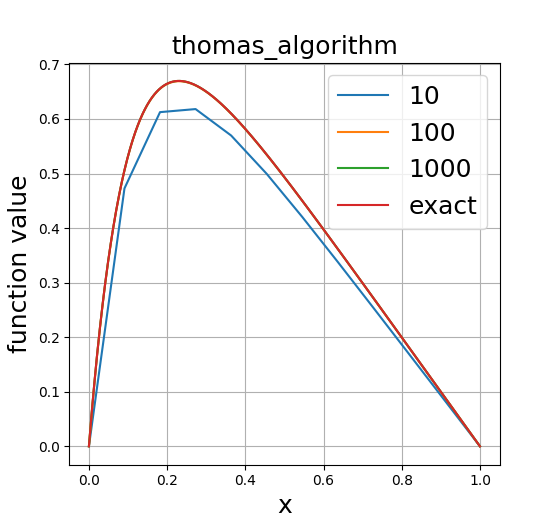
\includegraphics[scale=0.5]{thomas_data.png}
    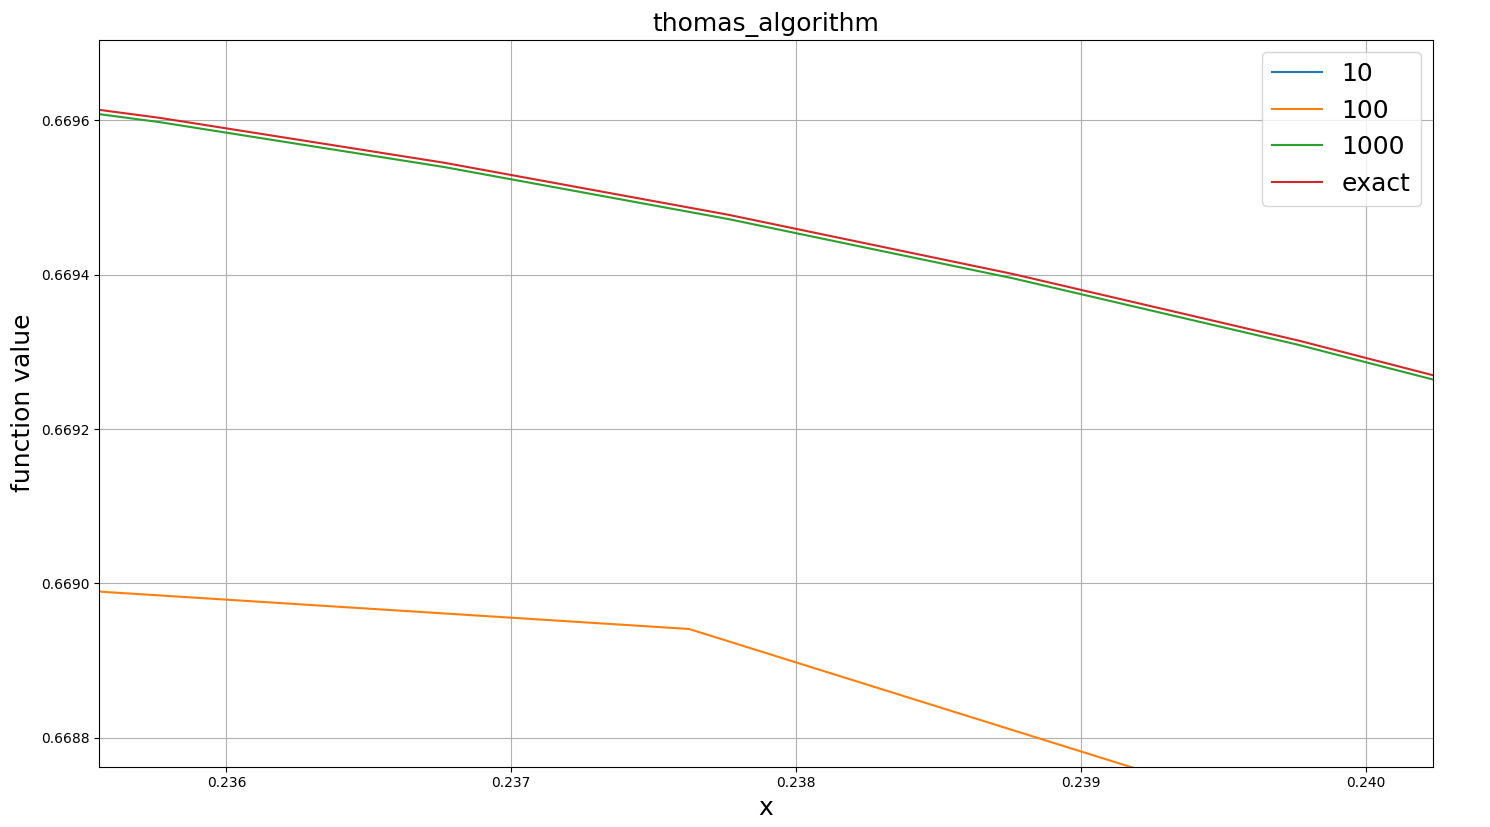
\includegraphics[scale=0.5]{thomas_data_zoom.png}
    \caption{Upper: The Thomas algorithm applied for 10, 100 and 1000 grid points on the interval $x \in [0, 1]$. The exact value is also plotted. Lower: The same data plotted, but zoomed in to see the that the lines lie close togehter.}
    \label{fig:thomas_data}
\end{figure}

%%%%%%%%%%%%%%%%%%%%%%%%%%%%%%%%%%%%
\subsection{Error analysis}
%%%%%%%%%%%%%%%%%%%%%%%%%%%%%%%%%%%%

Figure \ref{fig:error_data} shows the maximum relative error (\ref{eq:max_rel_error}) for the Thomas algorithm and the LU decomposition in a log-log-plot. The error plot for the specialized Thomas algorithm is not included since it looks exactly like the plot for the Thomas algorithm. We see that the error in the Thomas algorithm follows a straight line, with approximately a slope of 2, until it reaches \(n=10^{5}\). Here we see the numerical error increasing. The LU decomposition is an entirely different story. We see that the error varies extremely in the middle. We have not found out why. 

The points \(n=10,\,100\,1000\) is marked in both plots with red dots.

\begin{figure}[h]
    \centering
    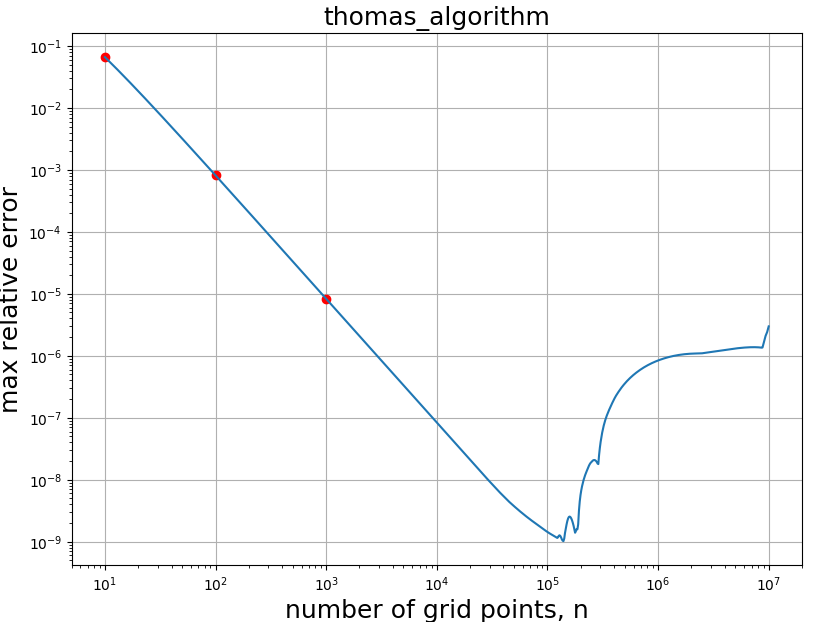
\includegraphics[scale=0.4]{error_data.png}
    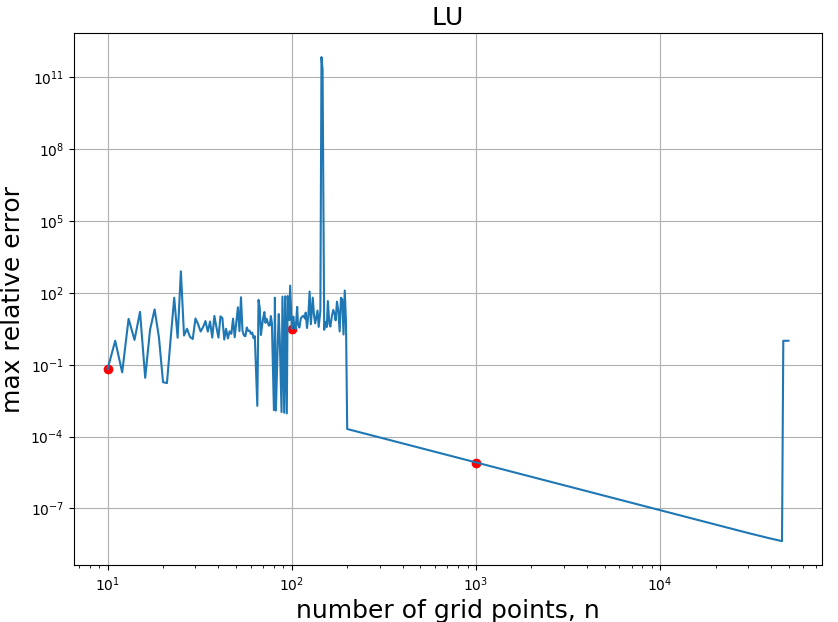
\includegraphics[scale=0.4]{error_data_LU.png}
    \caption{The figure shows how the algorithm increases linearly in precision in a log-log plot. The slope is approximately 2. After a given number of grid points (here approximately \(n=10^{5}\), the numerical error increases and takes over the analytical error. The same plot for the specialized Thomas algorithm gives the same result and is therefore not included. In the bottom plot we see how the maximum relative error for the LU decomposition does not give good results in the middle. We have not found out why, but we expect the mean to follow a more straight line. However, it does look like the error could follow a straight, but varies in the middle.}
    \label{fig:error_data}
\end{figure}

%%%%%%%%%%%%%%%%%%%%%%%%%%%%%%%%%%%%
\subsection{Time analysis}
%%%%%%%%%%%%%%%%%%%%%%%%%%%%%%%%%%%%

    Figure \ref{fig:algorithm_time} show the time usage in seconds for the three different algorithms in a log-log-plot. We can see how the two Thomas algorithms follows almost the same line with different slopes due to the different number of FLOPS that they use.
    
    What came to light pretty fast is that the LU decomposition is way too demanding to run anything as high as $10^5$ grid points. With a grid size of $10^5 \cdot 10^5$ we get a matrix with $10^{10}$ grid points. If each grid point holds an integer value of 16 bits, we need approximately 20GB of memory to store the matrix. If the computer does not have this much RAM, it will start storing the data in the swap file, which will slow down the computation significantly.
    
%Figure \ref{fig:algorithm_time} show the time usage in seconds for the three different algorithms in a log-log-plot. We can see how the two Thomas algorithms follows almost the same line with different slopes due to the different number of FLOPS that they use.
%
%What came to light pretty fast is that the LU decomposition is way too demanding to run anything as high as $10^5$ grid points. With a grid size of $10^5 \cdot 10^5$ we get a matrix with $10^{10}$ grid points. If each grid point holds an integer value of 16 bits, we need approximately 20GB of memory to store the matrix. If the computer does not have this much RAM, it will start storing the data in the swap file, which will slow down the computation significantly.
    
\begin{figure}[h]
    \centering
    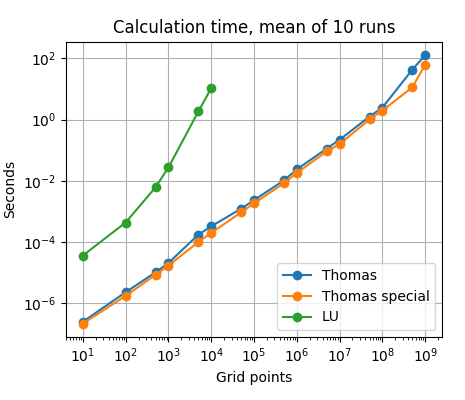
\includegraphics[scale=0.6]{algorithm_time.png}
    \caption{The figure shows the mean time usage for ten separate runs, of the three different algorithms in a logarithmic plot. The LU decomposition (and the solve method from armadillo) quickly increases in time usage (as expected because of the \(2/3n^{3} FLOPS\)) and above \(10^{4}\) grid points, it uses so much time that we choose to stop it. The Thomas algorithm (and the specialized one) looks linear with approximately a slope of 2, which is expected.}
    \label{fig:algorithm_time}
\end{figure}

%%%%%%%%%%%%%%%%%%%%%%%%%%%%%%%%%%%%
%%%%%%%%%%%%%%%%%%%%%%%%%%%%%%%%%%%%
\section{Discussion}
%%%%%%%%%%%%%%%%%%%%%%%%%%%%%%%%%%%%
%%%%%%%%%%%%%%%%%%%%%%%%%%%%%%%%%%%%

Our results show that the analysis is far from done. We would also like to improve our program, but we do not have time to do this. We will therefore focus on the result we have and explain how we could improve them.

%%%%%%%%%%%%%%%%%%%%%%%%%%%%%%%%%%%%
\subsection{Computed vs. exact solution}
%%%%%%%%%%%%%%%%%%%%%%%%%%%%%%%%%%%%

The data in figure \ref{fig:thomas_data} show that the numerical values approach the exact solution as $n$ gets larger. The bottom plot in figure \ref{fig:thomas_data} shows a zoomed version of the top figure, revealing that the numerical calculation for $n=1000$ is very close to the exact solution. Our results for the specialized Thomas algorithm and LU decomposition shows the exact same trend, and does not differ from the data in figure \ref{fig:thomas_data} in any significant way. This is expected, since the three algorithms are solving the exact same matrix equation, and they only differ by how many floating point operations they use per iteration, i.e., the time usage of the algorithms. 

%%%%%%%%%%%%%%%%%%%%%%%%%%%%%%%%%%%%
\subsection{Error analysis}
%%%%%%%%%%%%%%%%%%%%%%%%%%%%%%%%%%%%

From equation (\ref{eq:f_double_derivative_taylor}) we see that we expect an error proportional to \(h^{2}\). For a logarithmic scale this is equivalent to a line with slope 2 (as long as the proportionality constant does not change to much). From figure \ref{fig:error_data} we see that the Thomas algorithm follow this line almost perfectly up to \(n=10^{5}\). 

We know that the computer can only represent numbers to a finite decimal point. When \(n\) increases, we know that the step size \(h = \frac{1}{n}\) decreases. This introduces round-off errors, which for large \(n\) will make the discretized functions unstable.

The LU decomposition is a different story entirely; we see that the relative error varies extremely and is located far away from the line we expect to see. We are more or less doing the exact same thing when calculating the relative error for the Thomas algorithm as when we do it for the LU decomposition, and we have indeed yet to find out why this behaviour occurs as it does.

%shows the maximum relative error (\ref{eq:max_rel_error}) for the Thomas algorithm and the LU decomposition in a log-log-plot. The error plot for the specialized Thomas algorithm is not included since it looks exactly like the plot for the Thomas algorithm. We see that the error in the Thomas algorithm follows a straight line, with approximately a slope of 2, until it reaches \(n=10^{5}\). Here we see the numerical error increasing. The LU decomposition is an entirely different story. We see that the error varies extremely in the middle. We have not found out why. 

%%%%%%%%%%%%%%%%%%%%%%%%%%%%%%%%%%%%
\subsection{Time usage}
%%%%%%%%%%%%%%%%%%%%%%%%%%%%%%%%%%%%

%%%%%%%%%%%%%%%%%%%%%%%%%%%%%%%%%%%%
%%%%%%%%%%%%%%%%%%%%%%%%%%%%%%%%%%%%
\section{Conclusion}
%%%%%%%%%%%%%%%%%%%%%%%%%%%%%%%%%%%%
%%%%%%%%%%%%%%%%%%%%%%%%%%%%%%%%%%%%

% BIBLIOGRAPHY
\bibliography{referanser}
\bibliographystyle{aasjournal}
%\bibliographystyle{plain}

\end{document}
% Trenger referanser på poisson likning, dirichlet grensebetingelser, taylor-rekker (kap. 11 i kalkulus) og feilen fra taylor-tilnærming (kap. 9 i Knut Mørkens kompendium). Thomas algo og LU + flops til begge.

% kanskje for dirichlet boundary condition (?): https://www.researchgate.net/publication/222641921_Heritage_and_early_history_of_the_boundary_element_method